\documentclass[a4paper,12pt]{article}

\usepackage[T2A]{fontenc}
\usepackage[utf8]{inputenc}
\usepackage[english,russian]{babel}
\usepackage{amsmath}
\usepackage{pgfplots}
\usepackage{geometry}
\usepackage{graphicx}
\usepackage[section,above,below]{placeins}
\usepackage{afterpage,placeins}
\usepackage{booktabs}
\usepackage{listings}
\usepackage{color}

\usepackage{algorithm}
\usepackage[noend]{algpseudocode}

\DeclareGraphicsExtensions{.png,.jpg}

\geometry{left=2cm}
\geometry{right=1.5cm}
\geometry{top=1cm}
\geometry{bottom=1.5cm}

\headheight = 1cm
\footskip = 0.5cm

\parskip = 4.25mm % расстояние между строками
\parindent=6.375mm % расстояние между абзацами
\floatname{algorithm}{Алгоритм} % переопределение имени в псевдокоде

\begin{document}
\lstset{
	        		language=C++,
	        		basicstyle=\ttfamily,
	        		keywordstyle=\color{blue}\ttfamily,
	        		stringstyle=\color{red}\ttfamily,
	        		commentstyle=\color{green}\ttfamily,
	        		morecomment=[l][\color{magenta}]{\#},
	        		columns=fullflexible,
	        	    tabsize=1, 
	        		breakatwhitespace=true
	        	}
    \begin{titlepage}
        \begin{center}
            \large
            Государственное образовательное учреждение высшего  образования\\
            “Московский государственный технический университет имени Н.Э.Баумана”
            \vspace{3cm}
            
            \textsc{Дисциплина: Анализ алгоритмов}
            \vspace{0.5cm}
                
            \textsc{Лабораторная работа №7}
            \vspace{3cm}
            
            {\LARGE Алгоритмы поиска подстроки в строке}
            \vspace{3cm}
            
            Студент группы ИУ7-54Б,\\   
            Котов Никита
            \vfill
            
            2019 г.            
            \end{center}
    \end{titlepage}
    
    \begin{center}
    	\tableofcontents
    \end{center}
	
	\setcounter{page}{2}
	\newpage   

    \begin{center}
        \section{Аналитическая часть}
        \subsection{Цели и задачи работы}
    \end{center}
    
		Цель лабораторной работы: изучить алгоритмы поиска подстроки в строке. \\*
В рамках выполнения работы необходимо решить следующие задачи:
		\begin{itemize}
			\item изучить стандартный алгоритм, алгоритмы Кнута-Морриса-Пратта и Бойера-Мура;
			\item реализовать данные алгоритмы;
			\item привести подробное описание работы каждого алгоритма.
		\end{itemize}
    
    \begin{center}
	    \subsection{Описание алгоритмов}
    \end{center}
    
\textbf{Постановка задачи:} пусть даны строки \textit{source} и \textit{pattern}, обозначим их \textit{s} и \textit{p} соответственно.  
Необходимо проверить входит ли строка \textit{p} в \textit{s}, если да, то найти индекс первого вхождения.

\subsubsection{Стандартный алгоритм}
Стандартный алгоритм основан на последовательном сравнении всех подстрок строки \textit{s} с \textit{p}, т.е. будет происходить сравнение всех подстрок размера $|p|$, начиная с индексов $i = 1,2,...,|s|-|p|+1$.

Пусть $s= "abcabccba"$, $p = "cab"$. В таблце 1 показаны сравнения символов, выполняемые в ходе работы алгоритма.
\begin{table}[h]
	    		\caption{Таблица коэффициентов для класса данных №1}
	    		\begin{center}
	    			\begin{tabular}{|c|c|c|c|c|c|c|c|c|c|}
	    			\hline
	    			№&a&b&c&a&b&c&c&b&a\\
	    			\hline	    			
	    			1&c&a&b& & & & & &\\
	    			\hline	    			
	    			2& &c&a&b& & & & &\\
	    			\hline	    			
	    			3& & &c&a&b& & & &\\
	    			\hline	    			
	    			\end{tabular}
	    			\label{T:t1}	
	    		\end{center}
\end{table}

\textbf{Поэтапное описание алгоритма:}
\begin{enumerate}
\item $i = j = 0$, $i \in [0, |s|-1], j \in [0, |p| - 1]$.
\item Посимвольно сравниваем \textit{s} c \textit{p}, \textit{s[i]} c \textit{p[j]}.
\item Если найдено совпадение, то увеличиваем $i$ и $j$, если $j=|p|$, то подстрока найдена, иначе прикладываем \textit{p} к следующему символу \textit{s}.
\end{enumerate}
\newpage
В листинге 1 представлена реализация стандартного алгоритма.
\begin{lstlisting}[frame=single,caption=Стандартный алгоритм, breaklines]
int standart(const std::string &str, const std::string &substr) {
    const auto str_len = str.length();
    const auto sub_len = substr.length();

    for (size_t i = 0; i <= str_len - sub_len; i++) {
        auto tmp_i = i;
        for (size_t j = 0; j < sub_len; j++) {
            if (substr[j] != str[tmp_i]) {
                break;
            }
            if (j == sub_len - 1) {
                return static_cast<int>(i);
            }
            tmp_i++;
        }
    }

    return -1;
}
\end{lstlisting}

\subsubsection{Алгоритм Кнута-Морриса-Пратта}

Алгоритм Кнута-Морриса-Пратта является оптимизацией стандартного алгоритма. Необходимо дать определения префикса, суффикса и префикс-функции.

Префикс \textit{pf} строки \textit{s} - последовательность символов строки такая, что $pf=s[0,...,i), i \in [0, |s|-1]$.

Суффикс \textit{sf} строки \textit{s} - последовательность символов строки такая, что $sf=s[i,...,|s|-1], i \in [1, |s|-1]$.

Префикс-функция строки \textit{s} на позиции \textit{i} - функция, возвращающая длину \textit{k} наибольшего собственного префикса строки \textit{s}, совпадающего с суффиксом этой строки.

Пусть строка $s = "cbcbc"$, рассмотрим все ее суффиксы, префиксы и значения префикс-функции, представленные в таблице 2.

\begin{table}[h]
	    		\caption{Пример таблицы префиксов и суффиксов для строки s}
	    		\begin{center}
	    			\begin{tabular}{|c|c|c|c|}
	    			\hline
	    			i&Prefix(s,i)&префиксы&суффиксы\\
	    			0&0&c&c\\
	    			1&0&c&b\\
	    			2&1&c, cb&c, bc\\
	    			3&3&c, cb, cbc&c, bc, cbc\\
	    			4&3&c, cb, cbc, cbcb&c, bc, cbc, bcbc\\
	    			\hline
	    			\end{tabular}
	    			\label{T:t1}	
	    		\end{center}
\end{table}
\newpage
Данный алгоритм использует автомат, прикладывание искомой подстроки к строке происходит при помощи вспомогательного массива сдвигов.

Алгоритм заполнения массива сдвигов:
\begin{enumerate}
\item Создать массив $shift, |shift| = |p|$;
\item $shift|0| = 0$;
\item $i=1,j=0$ -- индексы для строки и массива сдвигов соответственно;
\item Сравниваем $p[i]$ и $p[j]$, при совпадении $shift[i] = j+1$, сдвигаемся на символ вперед; иначе если $j = 0$, длина префикса нулевая, то $shift[i] = 0$.
\item Если $j \neq 0$, то $j = shift[j-1]$.
\item Если просмотрена не вся строка, то возвращаемся на 4ый шаг.
\end{enumerate}

Шаблонная строка устанавливается в начало исходной, затем аналогично стандартному алгоритму проводтся посимвольное сравнение. При нахождении несоответствия выполняется сдвиг \textit{p} с помощью массива сдвигов. Таким образом удается снизить число сравнений.

Рассмотрим работу алгоритма на примере $s = "abacababda, p = "abab"$, см. рис. 1.
\begin{figure}[H]	
			 	{
			 		\centering
			 		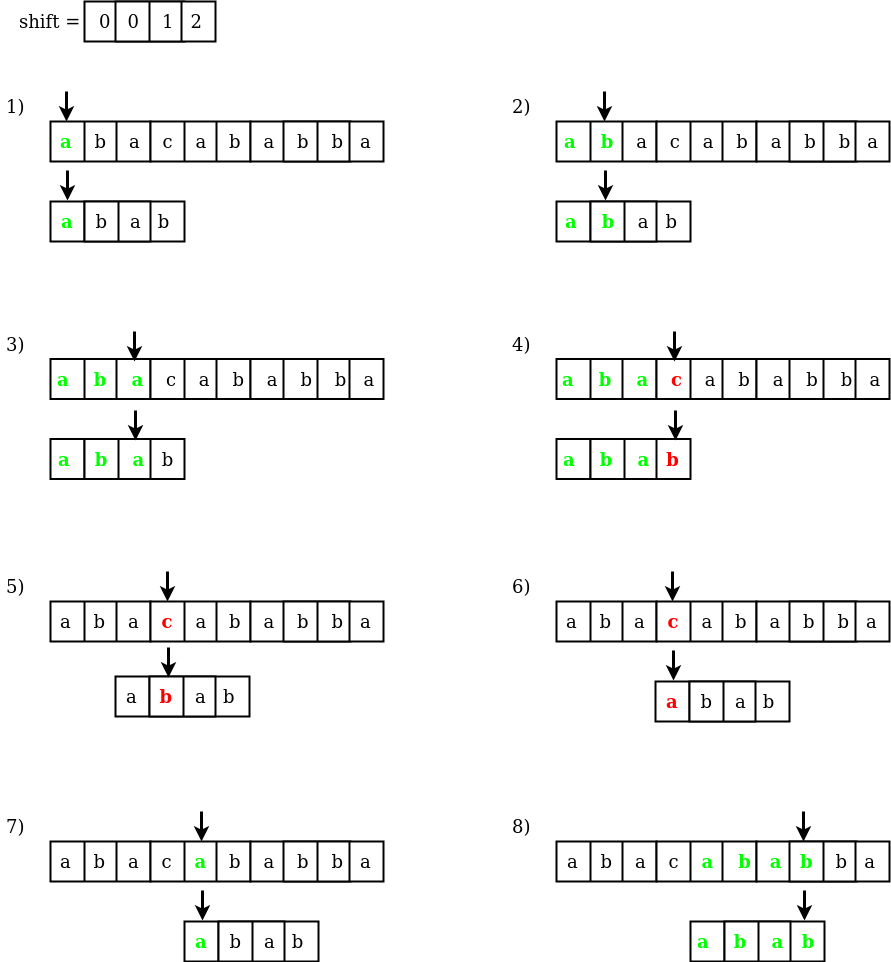
\includegraphics[scale=0.41]{1.png}
			 		\caption{Пример работы алгоритма Кнута-Морриса-Пратта.}
			 		\label{pic:ant_schema}
			 	}
			 \end{figure}

В листинге 2 представлена реализации алгоритма Кнута-Морриса-Пратта.
\begin{lstlisting}[frame=single,caption=Алгоритм Кнута-Морриса-Пратта, breaklines]
std::vector<size_t> get_shift(const std::string &str, const size_t &size) {
    std::vector<size_t> shift(size);
    shift[0] = 0;

    for (size_t i = 1; i < size; i++) {
        auto j = shift[i - 1];
        while (j > 0 && str[i] != str[j]) {
            j = shift[j - 1];
        }
        if (str[i] == str[j]) {
            j++;
        }
        shift[i] = j;
    }

    return shift;
}

int kmp(std::string str, std::string substr) {
    auto str_len = str.length();
    auto sub_len = substr.length();
    if (str_len < sub_len) {
        return -1;
    }

    std::vector<size_t> shift = get_shift(substr, sub_len);

    for (size_t j = 0, i = 0; i < str_len; i++) {
        while (j > 0 && str[i] != substr[j]) {
            j = shift[j - 1];
        }
        if (str[i] == substr[j]) {
            j++;
        }
        if (j == sub_len) {
            return static_cast<int>(i - j + 1);
        }
    }

    return -1;
}
\end{lstlisting}
\newpage
\subsubsection{Алгоритм Бойера-Мура}

Рассмотрим пошагово алгоритм Бойера-Мура:
\begin{enumerate}
\item Построить таблицу смещений для каждого символа.
\item Совмещение \textit{s} и \textit{p} по началу.
\item Сравнение символов справа налево. Если найдено несовпадение, то \textit{p} смещается вправо на число символов, взятое из таблицы смещений по символу исходной строки, иначе переходим к следующему символу.
\item Если просмотрена не вся исходная строка, то переход к пункту 3.
\end{enumerate}

Отдельно рассмотрим построение таблицы смещений. Необходимо построить ее так, чтобы пропустить максимально возможное количество незначащих символов. Для этого каждому символу ставится в соответствие величина, равная разности длины шаблона и порядкового номера символа (если символ повторяется, то берется самое правое вхождение, при этом последний символ не учитывается), что равносильно порядковому номеру символа, если считать его с конца строки. Это дает возможность смещаться вправо на максимальное число позиций.

На рис. 2 приведен пример генерации таблицы смещений символов для $s = "cbcbc"$.

\begin{figure}[H]	
			 	{
			 		\centering
			 		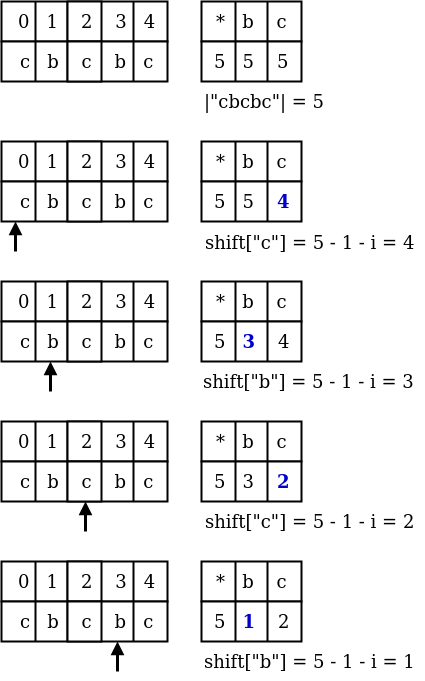
\includegraphics[scale=0.53]{2.png}
			 		\caption{Пример генерации таблицы сдвигов.}
			 		\label{pic:ant_schema}
			 	}
			 \end{figure}
			 
			 \newpage
На рис.3 приведен пример работы алгоритма Бойера-Мура при $s = "abcdefgabc", p = "efg"$.

\begin{figure}[H]	
			 	{
			 		\centering
			 		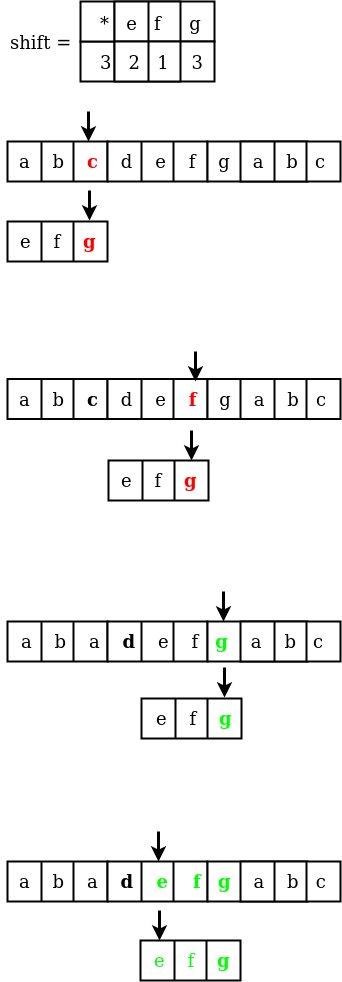
\includegraphics[scale=0.48]{3.png}
			 		\caption{Пример работы алгоритма Бойера-Мура.}
			 		\label{pic:ant_schema}
			 	}
			 \end{figure}
На листинге 3 представлена реализация алгоритма Бойера-Мура.
\begin{lstlisting}[frame=single,caption=Стандартный алгоритм, breaklines]
std::map<char, size_t> get_shift(const std::string &substr) {
    size_t alphabet_size = 256;
    auto sub_size = substr.length();
    std::map<char, size_t> shift;

    for (size_t symb = 0; symb < alphabet_size; ++symb) {
        shift[static_cast<char>(symb)] = sub_size;
    }

    for (size_t symb = 0; symb < sub_size - 1; ++symb) {
        shift[static_cast<char>(substr[symb])] = sub_size - symb - 1;
    }

    return shift;
}

int bm(std::string str, std::string substr) {
    auto str_len = str.length();
    auto sub_len = substr.length();
    if (str_len < sub_len) {
        return -1;
    }

    auto shift = get_shift(substr);
    auto start = sub_len - 1;
    auto i = start;
    auto j = start;
    auto k = start;

    while (j >= 0 && i < str_len) {
        j = start;
        k = i;
        while (j >= 0 && str[k] == substr[j]) {
            --k;
            --j;
        }

        i += shift[str[i]];
    }

    return static_cast<int>(k >= str_len - sub_len ? -1 : k + 1);
}
\end{lstlisting}
	\begin{center}
	\subsection{Вывод по аналитическому разделу}
	\end{center}	
	По итогам аналитического раздела были описаны стандартный алгоритм, алгоритм Кнута-Морриса-Пратта и алгоритм Бойера-Мура для нахождения подстроки в строке.

    \newpage

    \begin{center}
        \section*{Заключение}
        \addcontentsline{toc}{section}{Заключение}
    \end{center}
            \label{sec:ending}


        Таким образом, в ходе лабораторной работы были изучены, описаны и реализованы стандартный алгоритм, алгоритм Кнута-Морриса-Пратта и алгоритм Бойера-Мура для нахождения подстроки в строке. 

\end{document}
